\chapter{Arhitektura i dizajn sustava}

Kako bi se omogućio ispravan rad web aplikacije te interakcija između korisnika i nje potrebno je nekoliko osnovnih komponenata. To su:

	\begin{itemize}
		\item \textbf{Web preglednik}
		\item \textbf{Web aplikacija}
		\item \textbf{Web poslužitelj}
		\item \textbf{Baza podataka i njezin poslužitelj}		
	\end{itemize}

	\begin{figure}[H]
		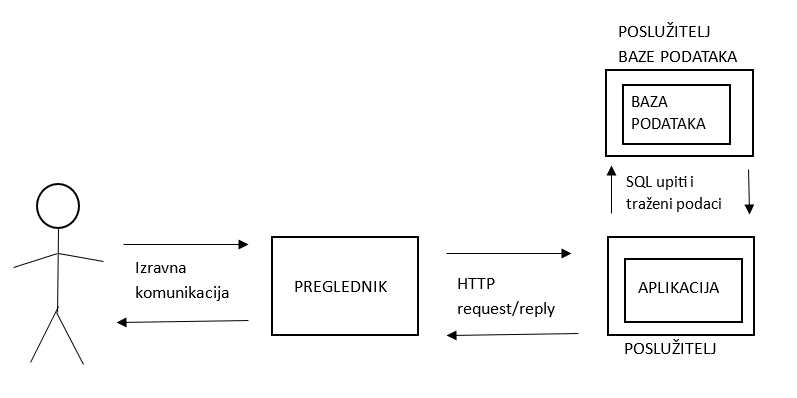
\includegraphics[scale=0.4]{slike/komunikacijaKomponenata.PNG}
		\centering
		\caption{Prikaz komunikacije između navedenih dijelova sustava}
		\label{fig:skicaKomunijacije}
	\end{figure}

	
	Web preglednik (klijent) šalje zahtjeve poslužitelju te prima odgovore kako bi prikazao sadržaj potreban korisniku. Nakon što dohvati programski kod te označni (markup) tekst potreban za prikaz web stranice, on prevodi taj kod i prikazuje ga korisniku na unaprijed definiran način. Način na koji će preglednik prikazati određeni element ili strukturu markup teksta nije propisan samim markup kodom, već ga određuje sam preglednik. Osim osnovnog koda stranice (.html), preglednik dohvaća i .css i .js datoteke te multimedijske sadržaje kao što su slike, videozapisi, zvuk i sl. \vspace{\baselineskip}
	
Sama komunikacija između preglednika i poslužitelja odvija se protokolom HTTP (Hypertext transfer protokol). Nakon što poslužitelj primi HTTP zahtjev, prosljeđuje ga web aplikaciji koja ga zatim obrađuje. Rezultat obrade se, nakon toga, vraća poslužitelju, koji ga prosljeđuje natrag korisniku u obliku HTTP odgovora. Tijekom obrade zahtjeva, ovisno o njegovoj prirodi, web aplikacija ponekad treba pristupiti bazi podataka. Bazi podataka se pristupa putem upita (npr. SQL). Koristit ćemo relacijsku bazu podataka i sustav PostgreSQL. Naime, s navedenom vrstom baza smo najbolje upoznati i imamo najviše iskustva u radu s njima. Osim toga, smatramo da nam omogućava ostvarenje svih planiranih funkcionalnosti potrebnih za našu aplikaciju. PostgreSQL se također temelji na modelu klijent – poslužitelj. Poslužitelj je u ovom slučaju povezan s bazom podataka te prima upite koje šalje web aplikacija. Server ih procesuira, pribavlja tražene informacije iz baze podataka te ih šalje aplikaciji. Aplikacija tada može dovršiti započetu operaciju tj. obraditi zahtjev korisnika/preglednika. \vspace{\baselineskip}

Za izradu aplikacije koristit ćemo programski jezik Java. Naime, to je jezik s kojim je većina članova našeg tima najbolje upoznata. Kako bismo ostvarili funkcionalnost backenda za našu aplikaciju, uz programski jezik Java koristit ćemo Spring radni okvir (framework). Za frontend ćemo koristiti JavaScript i njegov React library koji će nam omogućiti jednostavniju i elegantniju izradu web stranice. \vspace{\baselineskip}

Arhitektura sustava temeljit će se na MVC konceptu (model-controller-view). Ovaj način razvoja aplikacije ima brojne prednosti, ponajviše glede odvojenog razvoja dijelova aplikacije. S obzirom na to da su odgovornosti razdvojene kad se primjenjuje ova arhitektura, mnogo je lakše zasebno razvijati svaki dio te ga testirati odvojeno od ostalih. Olakšano je pronalaženje pogrešaka u programskom kodu te vršenje izmjena nad postojećim dijelovima projekta, bez većeg kompromitiranja postojećih funkcionalnosti. Osim toga, ovakav pristup olakšao bi rad na skalabilnosti aplikacije, ako bi to bilo potrebno u bilo kojem trenutku. Još jedan od razloga za korištenje arhitekture temeljene na MVC načelu je činjenica da ju podržava Spring radni okvir koji koristimo. Dijelovi ove arhitekture su sljedeći:

\begin{itemize}
\item \textbf{Model} – obuhvaća logiku i funkcionalnost aplikacije u smislu obrade podataka i upravljanja istima. Prima podatke od controllera i na temelju toga izvršava potrebne radnje nad podatcima te vraća rezultat natrag.

\item \textbf{Controller} – poveznica između model i view komponenata. Prihvaća zahtjeve poslane od strane korisnika te određuje kako odgovoriti na njih. Te informacije prosljeđuje modelu. Kad od modela dobije odgovor, rezultat obrade vraća korisniku putem view komponente. Podatci koje controller dobiva od korisnika mogu biti klikovi na gumbe, poslani obrasci i sl.

\item \textbf{View} – odnosi se na front end stranu aplikacije. To su dijelovi aplikacije koje korisnik vidi i s kojima izravno komunicira. View pribavlja podatke od modela te ih prikazuje na zaslonu računala na način razumljiv čovjeku. To su HTML, CSS datoteke i JS skripte na strani klijenta. 
\end{itemize}		
				
		\section{Baza podataka}
			
			\textbf{\textit{dio 1. revizije}}\\
			
			\textit{Potrebno je opisati koju vrstu i implementaciju baze podataka ste odabrali, glavne komponente od kojih se sastoji i slično.}
		
			\subsection{Opis tablica}
			
			\begin{center}
				\vspace{1cm}
				\begin{tabular}{ |p{4cm}|p{3cm}|p{5cm}|  }
					\hline
					\multicolumn{3}{|c|}{\textbf{ponuditelj}} \\
					\bottomrule[2pt]
					\cellcolor{green!25}korisnickoIme & VARCHAR &Skup znakova koji se koriste za prepoznavanje i pristup\\
					\hline
					lozinka & VARCHAR & Lozinka se koristi u kombinaciji s korisničkim imenom\\
					\hline
					e-posta & VARCHAR & Način kontaktiranja\\
					\hline
					adresa & VARCHAR & Podatci o mjestu na kojem ponuditelj radi\\
					\hline
					brojTelefona & INT & Način kontaktiranja\\
					\hline
				\end{tabular}
				\vspace{1cm}
				\begin{tabular}{ |p{4cm}|p{3cm}|p{5cm}|  }
					\hline
					\multicolumn{3}{|c|}{\textbf{knjige}} \\
					\bottomrule[2pt]
					\cellcolor{green!25}id & INT &Koristi za identifikaciju knjige\\
					\hline
					naziv & VARCHAR & Naslov knjige\\
					\hline
					autor & VARCHAR & Autor knjige\\
					\hline
					godinaIzdanja & INT & Godina izdanja\\
					\hline
					kategorijaIzdavaca & ENUM & Postoji dvije kategorije izdavača: domaći,strani\\
					\hline
					zanr & VARCHAR & Oblik književnog djela\\
					\hline
					ISBN & INT & Medunarodni standardni književni broj jedinstveni je identifikator knjiga\\
					\hline
					brojIzdanja & INT & Broj izdanja\\
					\hline
					stanjeOcuvanosti & VARCHAR & Stanje očuvanosti\\
					\hline
					tekstniOpis & VARCHAR & Sadržaj knjige\\
					\hline
					slikaKorica & IMAGE & Slika korica knjige\\
					\hline
					oznakaVrsteKnjige & ENUM & Oznaka vrste knjige može biti: strani-jezik, hrvatski-jezik-dobavljiva, hrvatski-jezik-nedobavljiva, srodni-jezik-nedobavljiva, srodni-jezik-dobavljiva\\
					\hline
					izdavac & VARCHAR & Naziv izdavača\\
					\hline
				\end{tabular}
				\vspace{1cm}
				\begin{tabular}{ |p{4cm}|p{3cm}|p{5cm}|  }
					\hline
					\multicolumn{3}{|c|}{\textbf{listaPonuda}} \\
					\bottomrule[2pt]
					\cellcolor{blue!10}id & INT & Koristi za identifikaciju knjige\\
					\hline
					brojDostupnihPrimjeraka & INT & Trenutni broj dostupnih primjeraka od odredenog ponuditelja\\
					\hline
					cijenaKnjige & FLOAT & Cijena knjige\\
					\hline
				\end{tabular}
				\vspace{1cm}
				\begin{tabular}{ |p{4cm}|p{3cm}|p{5cm}|  }
					\hline
					\multicolumn{3}{|c|}{\textbf{zahtjev}} \\
					\bottomrule[2pt]
					\cellcolor{blue!10}id & INT &Koristi za identifikaciju knjige\\
					\hline
				\end{tabular}
				\vspace{1cm}
				\begin{tabular}{ |p{4cm}|p{3cm}|p{5cm}|  }
					\hline
					\multicolumn{3}{|c|}{\textbf{ponuditi}} \\
					\bottomrule[2pt]
					\cellcolor{blue!10}id & INT & Koristi za identifikaciju knjige\\
					\hline
					\cellcolor{blue!10}korisnickoIme & VARCHAR & Skup znakova koji se koriste za prepoznavanje i pristup\\
					\hline
				\end{tabular}
				\vspace{1cm}
				\begin{tabular}{ |p{4cm}|p{3cm}|p{5cm}|  }
					\hline
					\multicolumn{3}{|c|}{\textbf{dostupni}} \\
					\bottomrule[2pt]
					\cellcolor{blue!10}korisnickoIme & VARCHAR & Skup znakova koji se koriste za prepoznavanje i pristup\\
					\hline
				\end{tabular}
				\vspace{1cm}
				\begin{tabular}{ |p{4cm}|p{3cm}|p{5cm}|  }
					\hline
					\multicolumn{3}{|c|}{\textbf{izdavac}} \\
					\bottomrule[2pt]
					\cellcolor{blue!10}korisnickoIme & VARCHAR & Skup znakova koji se koriste za prepoznavanje i pristup\\
					\hline
				\end{tabular}
				\vspace{1cm}
				\begin{tabular}{ |p{4cm}|p{3cm}|p{5cm}|  }
					\hline
					\multicolumn{3}{|c|}{\textbf{antikvarijat}} \\
					\bottomrule[2pt]
					\cellcolor{blue!10}korisnickoIme & VARCHAR & Skup znakova koji se koriste za prepoznavanje i pristup\\
					\hline
				\end{tabular}
				\vspace{1cm}
				\begin{tabular}{ |p{4cm}|p{3cm}|p{5cm}|  }
					\hline
					\multicolumn{3}{|c|}{\textbf{preprodavac}} \\
					\bottomrule[2pt]
					\cellcolor{blue!10}korisnickoIme & VARCHAR & Skup znakova koji se koriste za prepoznavanje i pristup\\
					\hline
				\end{tabular}
			\end{center}	
			
				
			
			\subsection{Dijagram baze podataka}
			
				\begin{figure}[H]
					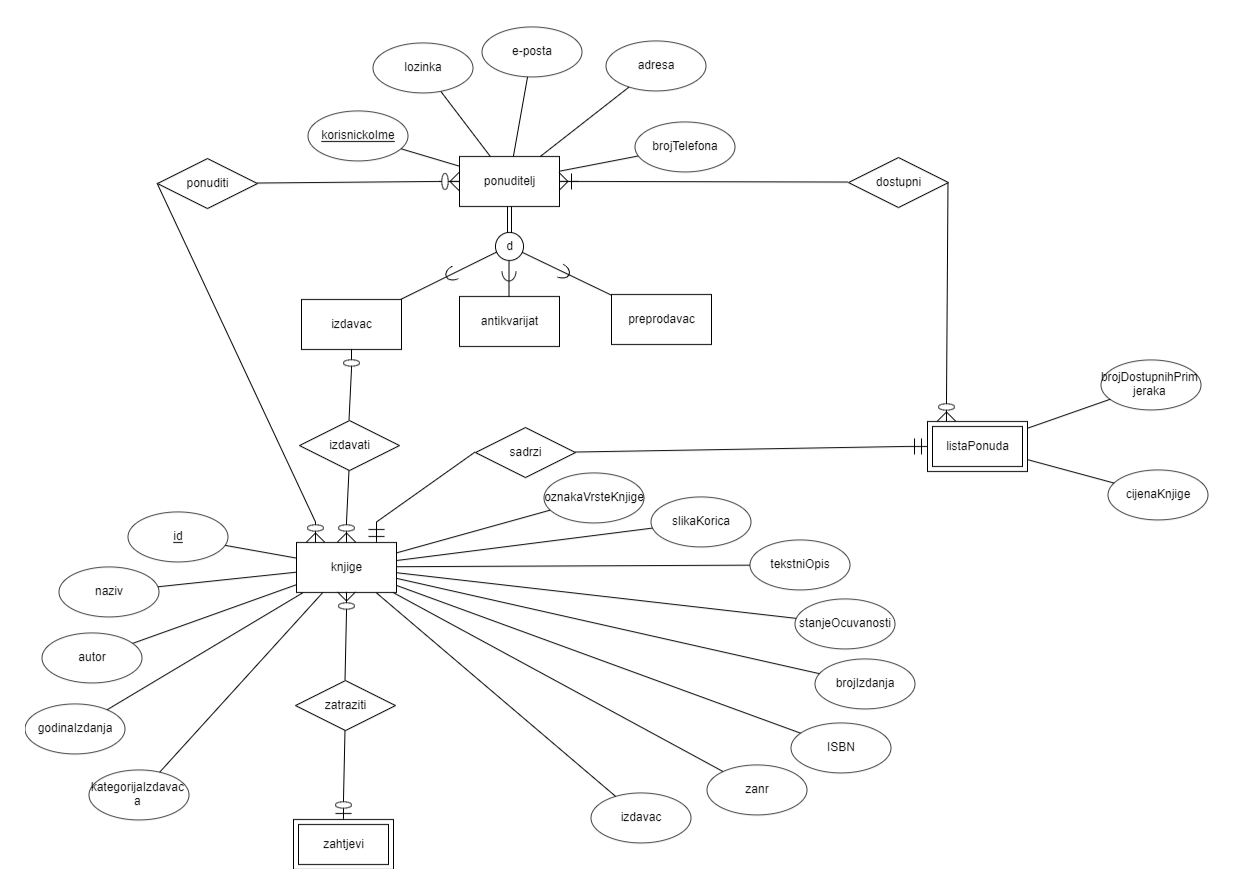
\includegraphics[scale=0.35]{slike/4.1.2 er_dijagram.PNG} %veličina slike u odnosu na originalnu datoteku i pozicija slike
					\centering
					\caption{ER dijagram}
					\label{fig:ER dijagram}
				\end{figure}
			
			\eject
			
			
		\section{Dijagram razreda}
		
			\textit{Potrebno je priložiti dijagram razreda s pripadajućim opisom. Zbog preglednosti je moguće dijagram razlomiti na više njih, ali moraju biti grupirani prema sličnim razinama apstrakcije i srodnim funkcionalnostima.}\\
			
			\textbf{\textit{dio 1. revizije}}\\
			
			\textit{Prilikom prve predaje projekta, potrebno je priložiti potpuno razrađen dijagram razreda vezan uz \textbf{generičku funkcionalnost} sustava. Ostale funkcionalnosti trebaju biti idejno razrađene u dijagramu sa sljedećim komponentama: nazivi razreda, nazivi metoda i vrste pristupa metodama (npr. javni, zaštićeni), nazivi atributa razreda, veze i odnosi između razreda.}\\
			
			\textbf{\textit{dio 2. revizije}}\\			
			
			\textit{Prilikom druge predaje projekta dijagram razreda i opisi moraju odgovarati stvarnom stanju implementacije}
			
			
			
			\eject
		
		\section{Dijagram stanja}
			
			
			\textbf{\textit{dio 2. revizije}}\\
			
			\textit{Potrebno je priložiti dijagram stanja i opisati ga. Dovoljan je jedan dijagram stanja koji prikazuje \textbf{značajan dio funkcionalnosti} sustava. Na primjer, stanja korisničkog sučelja i tijek korištenja neke ključne funkcionalnosti jesu značajan dio sustava, a registracija i prijava nisu. }
			
			
			\eject 
		
		\section{Dijagram aktivnosti}
			
			\textbf{\textit{dio 2. revizije}}\\
			
			 \textit{Potrebno je priložiti dijagram aktivnosti s pripadajućim opisom. Dijagram aktivnosti treba prikazivati značajan dio sustava.}
			
			\eject
		\section{Dijagram komponenti}
		
			\textbf{\textit{dio 2. revizije}}\\
		
			 \textit{Potrebno je priložiti dijagram komponenti s pripadajućim opisom. Dijagram komponenti treba prikazivati strukturu cijele aplikacije.}